\section{Laboratory work implementation}

\subsection{Tasks and Points}

În lucrarea de laborator dată au fost realizate următoarele sarcini:
\begin{enumerate}
\textbf{Advanced Level (nota 9 - 10):}
Dezvoltarea unei aplicatii:

\begin{enumerate}
\item  Mobile
\item  Web
\item  Browser Extension
\item  Game development (web, mobile, desktop)
\item  Service application
\item  Internet application
\item  Client application
\end{enumerate}Desktop


\subsection{Analiza lucrarii de laborator}

https://github.com/MarinaJechiuTI154/MIDPS
	
	Pentru crearea acestui proiect, membrii echipei au avut următoarele responsabilități:

	Cobîlaș Vasile
	\begin{itemize}
	\item crearea front-end-ului;
	\end{itemize}
	
	Popușoi Victor
	\begin{itemize}
	\item implementarea algoritmului jocului Yahtzee;
	\item crearea posibilitatii de inregistrare,logare,logout a utilizatorului;
	\item salvarea datelor despre utilizator in baza de date;
	\end{itemize}
	
	Jechiu Marina
	\begin{itemize}
	\item salvarea rezultatelor jocului în baza de date;
	\item crearea paginii Top 10 players;
	\item crearea paginii de contacte;
	\item efectuarea merge-ului și rezolvarea conflictelor;
	\end{itemize}
	
	În lucrare de laborator nr.5 s-a realizat un joc care se numește Yahtzee .
Este un joc cu zaruri unde scopul principal este acumularea a cât mai multe puncte, facând diferite
combinații de zaruri. Este considerat un joc extrem de ușor și foarte relaxant. Sunt 5 zaruri,
3 incercări și 13 combinații.Fiecare combinație validă de zaruri are un punctaj
diferit, unele combinații au un număr fix de puncte, iar altele au un număr de puncte egal cu suma
valorilor de pe zaruri. Subjocul Yahtzee înseamnă că jucătorul să aibă cinci zaruri la fel, de aceeași valoare, fiind cel mai bine punctată combinație din joc, valoarea punctelor castigate fiind de 50.

	Salvarea rezultatelor jocului se efectuează la sfârșitul jocului în baza de date yahtzee, în tabelul results. Acest tabel conține 3 câmpuri: id, username și score. Usernam-ul este dat de valoarea curentă a useru-ului logat, iar rezultatul de punctajul total ales de acesta. 
	
	Pagina de top conține un tabel din 10 câmpuri, care extrage rezultatele cele mai mari ale jucătorilor, obținute în urma jocului. Dacă în tabelul results apar noi date, tabelul cu topul se actualizează la un refresh al paginii.
	
	Pagina de contacte conține datele de contact ale administratorilor și o secțiune ce permite transmiterea feedback-urilor sub formă de mesaje.

	
\subsection{Imagini}
% Exemplu de figura cu titlu, si referinta, label

\begin{figure}[!ht]
\centering
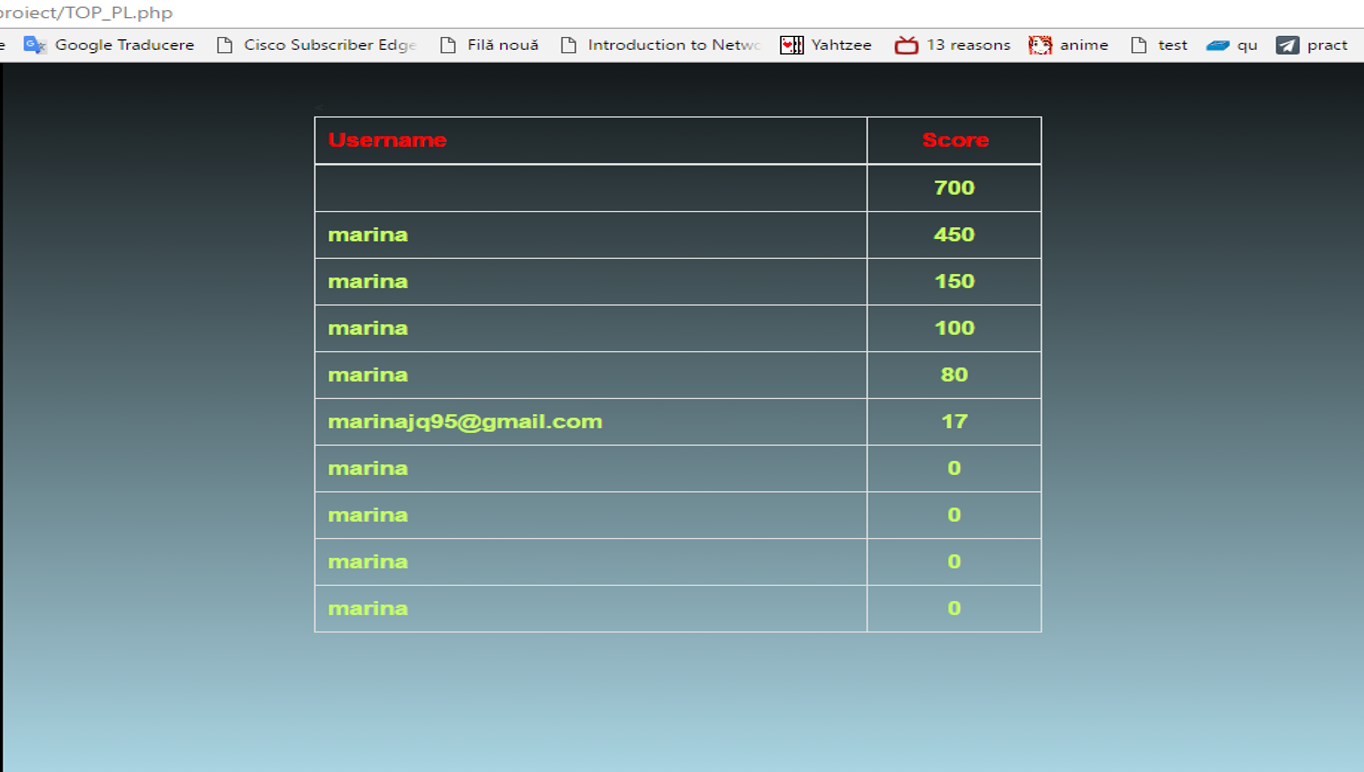
\includegraphics[width=1.0\textwidth]{1}
\caption{Pagina top players}

\end{figure}


\begin{figure}[!ht]
\centering

\includegraphics[width=1.0\textwidth]{2}
\caption{Pagina de contacte}

\end{figure}

\begin{figure}[!ht]
\centering
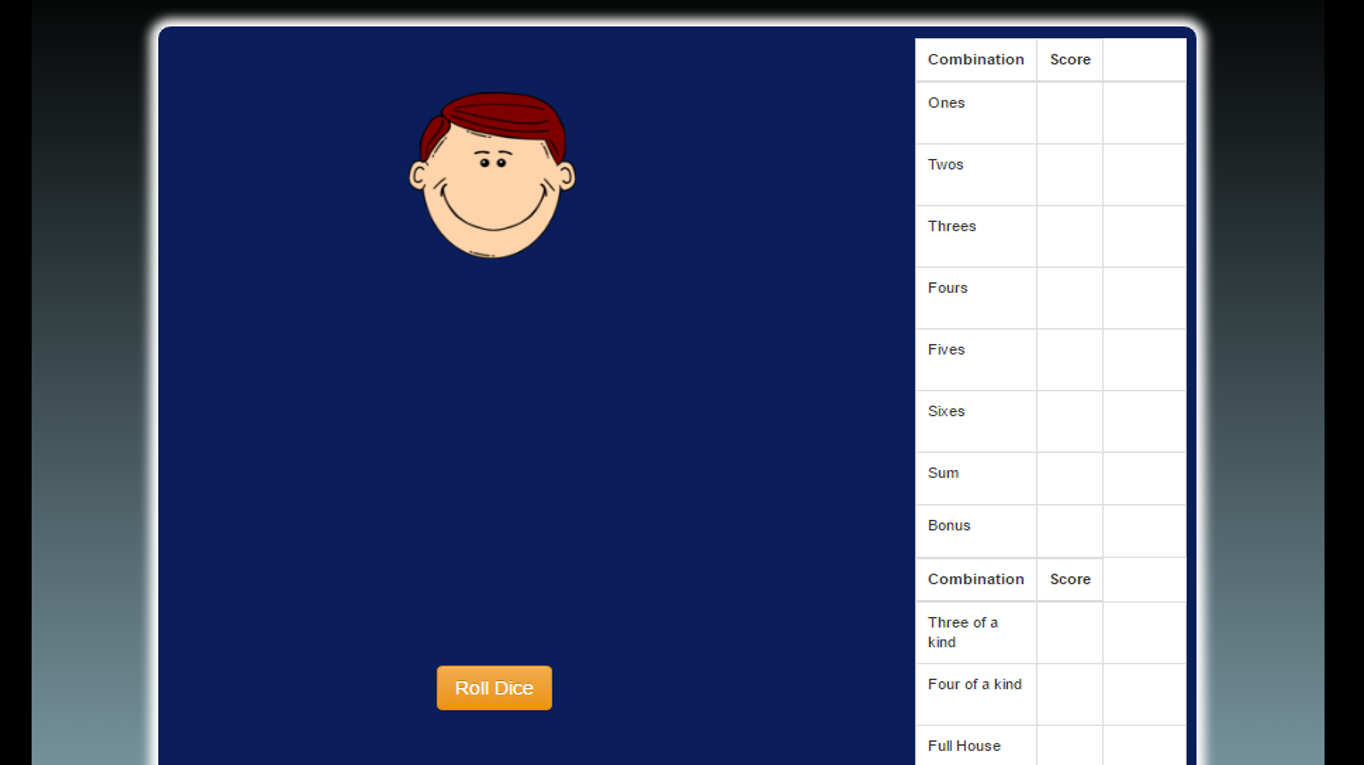
\includegraphics[width=1.0\textwidth]{3}
\caption{Pagina de joc}

\end{figure}

\begin{figure}[!ht]
\centering

\includegraphics[width=1.0\textwidth]{4}
\caption{Pagina about}

\end{figure}

% Exemplu de listing. Cum sa adaugi cod sursa in functie de limbajul de programare



% Exemplu de tabel. El poate fi efectuat si exportat in forma online: 
% http://www.tablesgenerator.com/






\clearpage